\section{Improving Load, Performance and Stress Evolutionary Testing using a Hybrid Metaheuristic Approach}

A  Load, Performance or Stress tests uses set of workloads that consists of many types of usage scenarios and different user numbers combinations. A load is typically based on an operational profile. For example,  The Fig. \ref{fig:example} shows an example  of a system under test with three pages (Main Page, Profile Page and Search Page) and six possible users. From the combinations of users and application pages various scenarios can be created as the scenarios 1 and 2 presented in the figure. The first scenario presents a test that has passed and the second scenario a test that had an http error 404.

\begin{figure}[ht]
\centering
\caption{Possible test scenarios for a hypothetical application}
\includegraphics[width=0.4\textwidth]{./images/diagram.png}
\label{fig:example}
\end{figure}


A performance test usually lasts for several hours or even a few days and only tests a limited number of workloads. The major challenge is to find the workloads  that exposes a major number of errors and discover the maximum number of users supported by a application under test \cite{Barna2011}. 


The main objective of the research is to find in a given search space as many users that supports an application under test for a given maximum response time.



\begin{figure}[ht]
\centering
\caption{Best results obtained in 27 generations}
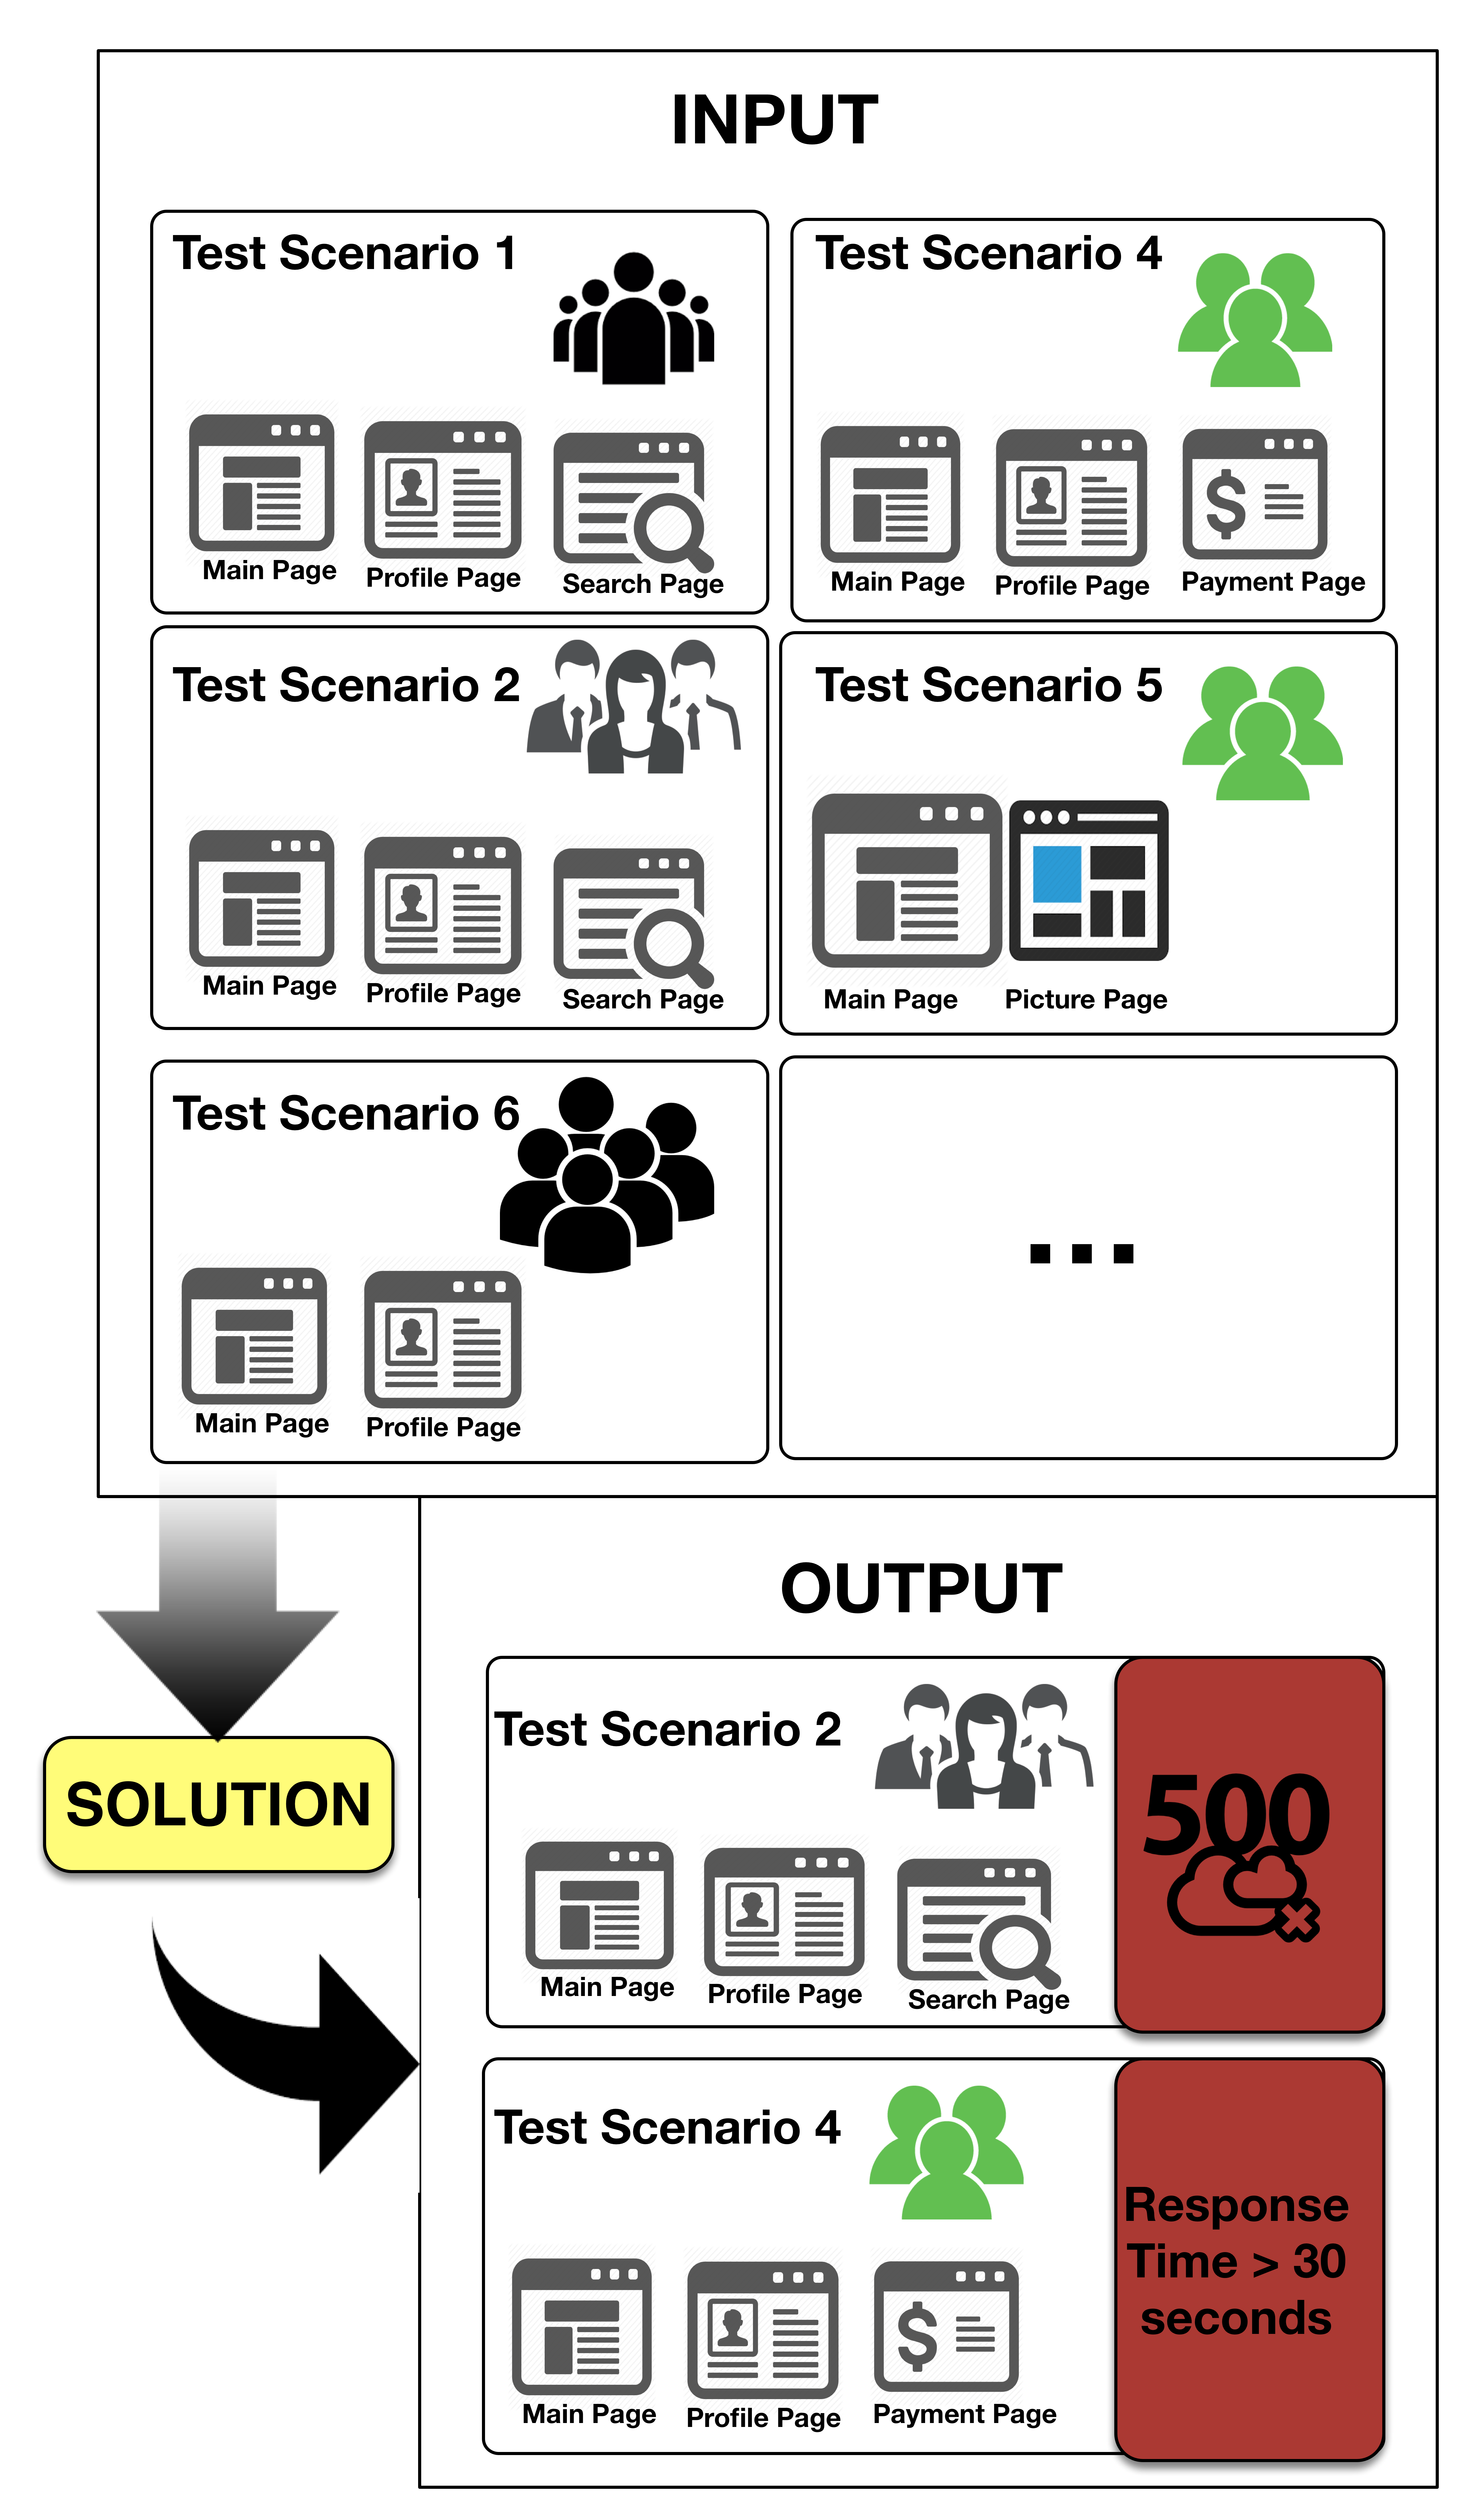
\includegraphics[width=0.5\textwidth]{./images/solution.png}
\label{fig:example}
\end{figure}


The proposed solution makes it possible to create a generative model that evolves during the test. The proposed solution model uses Genetic Algorithm, Tabu Search and Simulated Annealing in two different approaches.  The first approach uses the three algorithms independently and the second approach uses the three algorithms collaboratively (Hybrid Metaheuristic approach).

In the first approach , the algorithms do not share their best individuals among themselves. Each algorithm evolves in a separate way (Fig. \ref{fig:firstaproach}). The second approach use the algorithms in a collaborative mode (Hybrid Metaheuristic). In this approach, the three algorithms share their best individuals found (Fig. \ref{fig:secondapproach}).

The next subsections present details about the used metaheuristcs algorithms (genotype representation and fitnesse function) and the IAdapter components.

\begin{figure}[h]
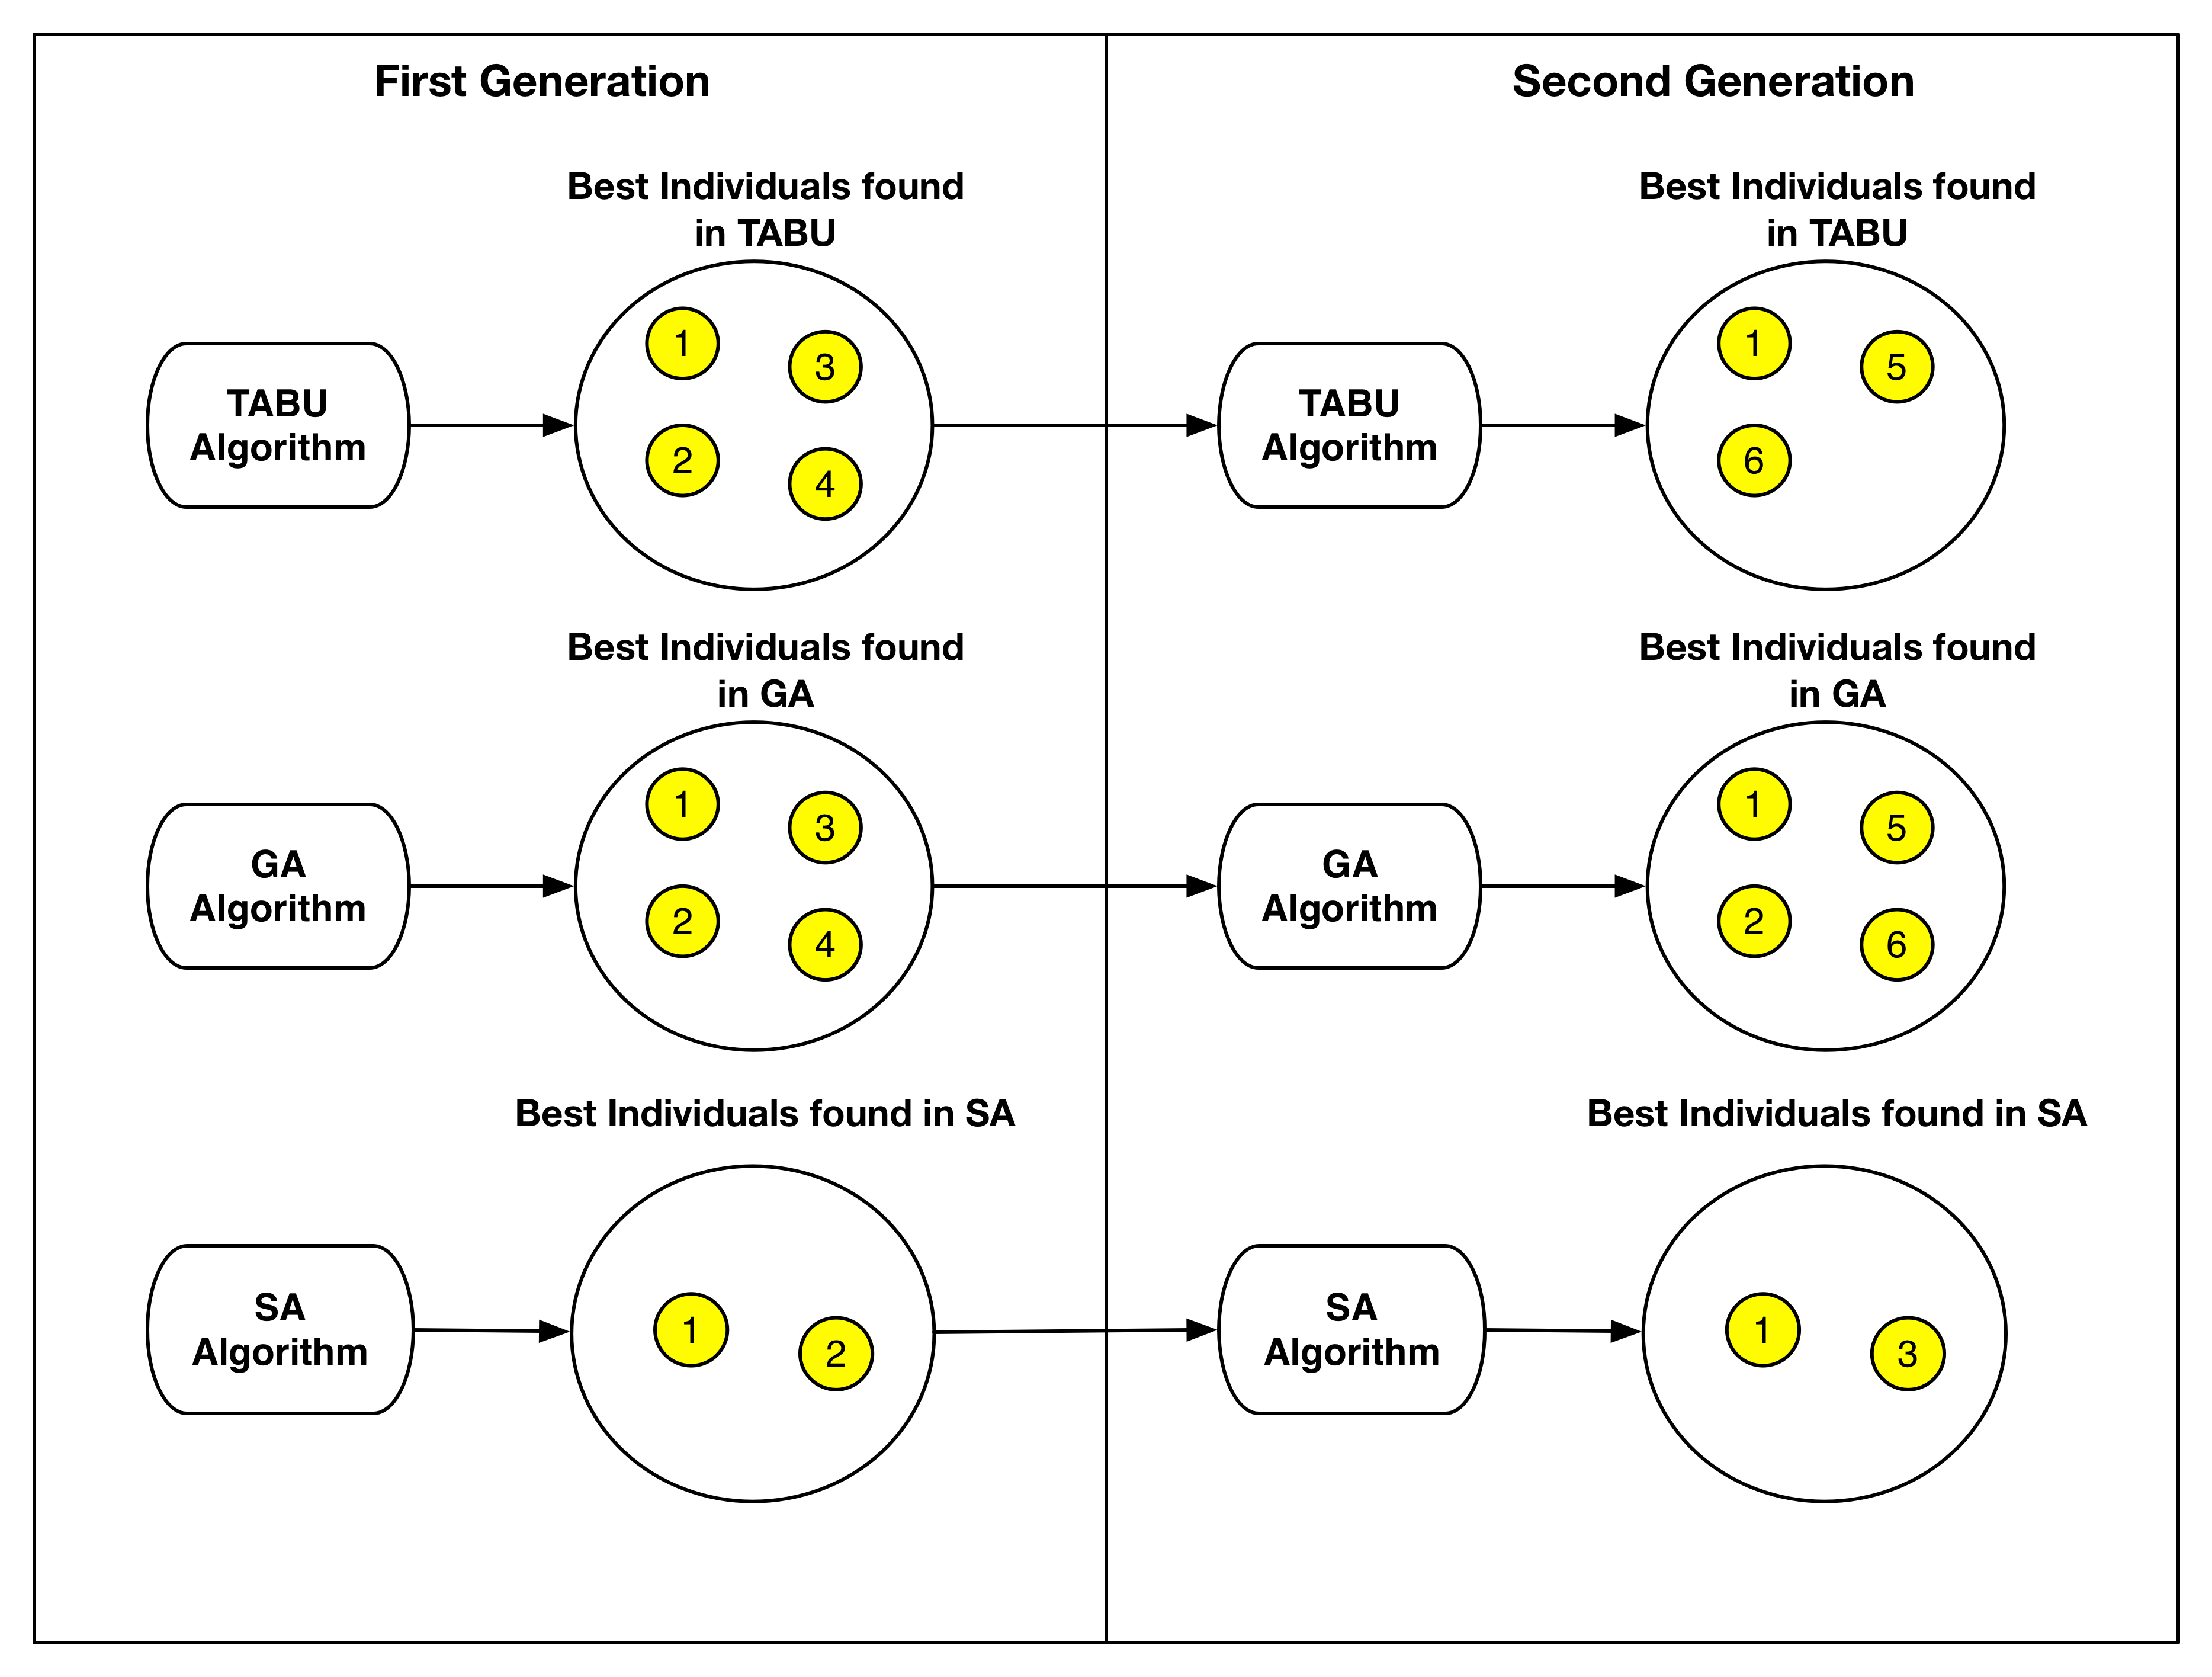
\includegraphics[width=0.5\textwidth]{./images/independ.png}
\caption{Use of the algorithms independently}
\label{fig:firstaproach}
\end{figure}
\begin{figure}
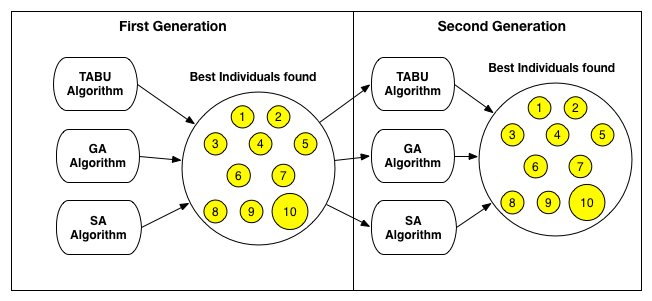
\includegraphics[width=0.5\textwidth]{./images/collaborative.png}
\caption{Use of the  algorithms collaboratively}
\label{fig:secondapproach}
\end{figure}

\subsection{Genotype representation}

The Genotype representation is composed by a linear vector with 23 genes. The first gene represents the name of individual. The second gene presents the  algorithm (Genetic Algorithm, Simulated Annealing or Tabu Search) used by the individual. The third gene represents the type of test (Load, Stress or Performance). Next genes represent 10 scenarios and their numbers of users. Each scenario is an atomic operation, the scenario must log in the application, run the task goal and undo any changes performed, returning the application to it's original state. 

The Fig. \ref{fig:genomarepresentation} presents the genome representation and  a example using the crossover operation. In the example, the genotype 1 has the Login scenario with 2 users; the Form scenario with 0 users and the Search scenario with 3 users. The genotype 2 has the Delete scenario with 10 users; the Search scenario with 0 users and the Include scenario with 5 users. After the crossover operation, We obtain a genotype with  Login scenario with 2 users; the Search scenario with 0 users and the Include scenario with 5 users.

\begin{figure}[h]
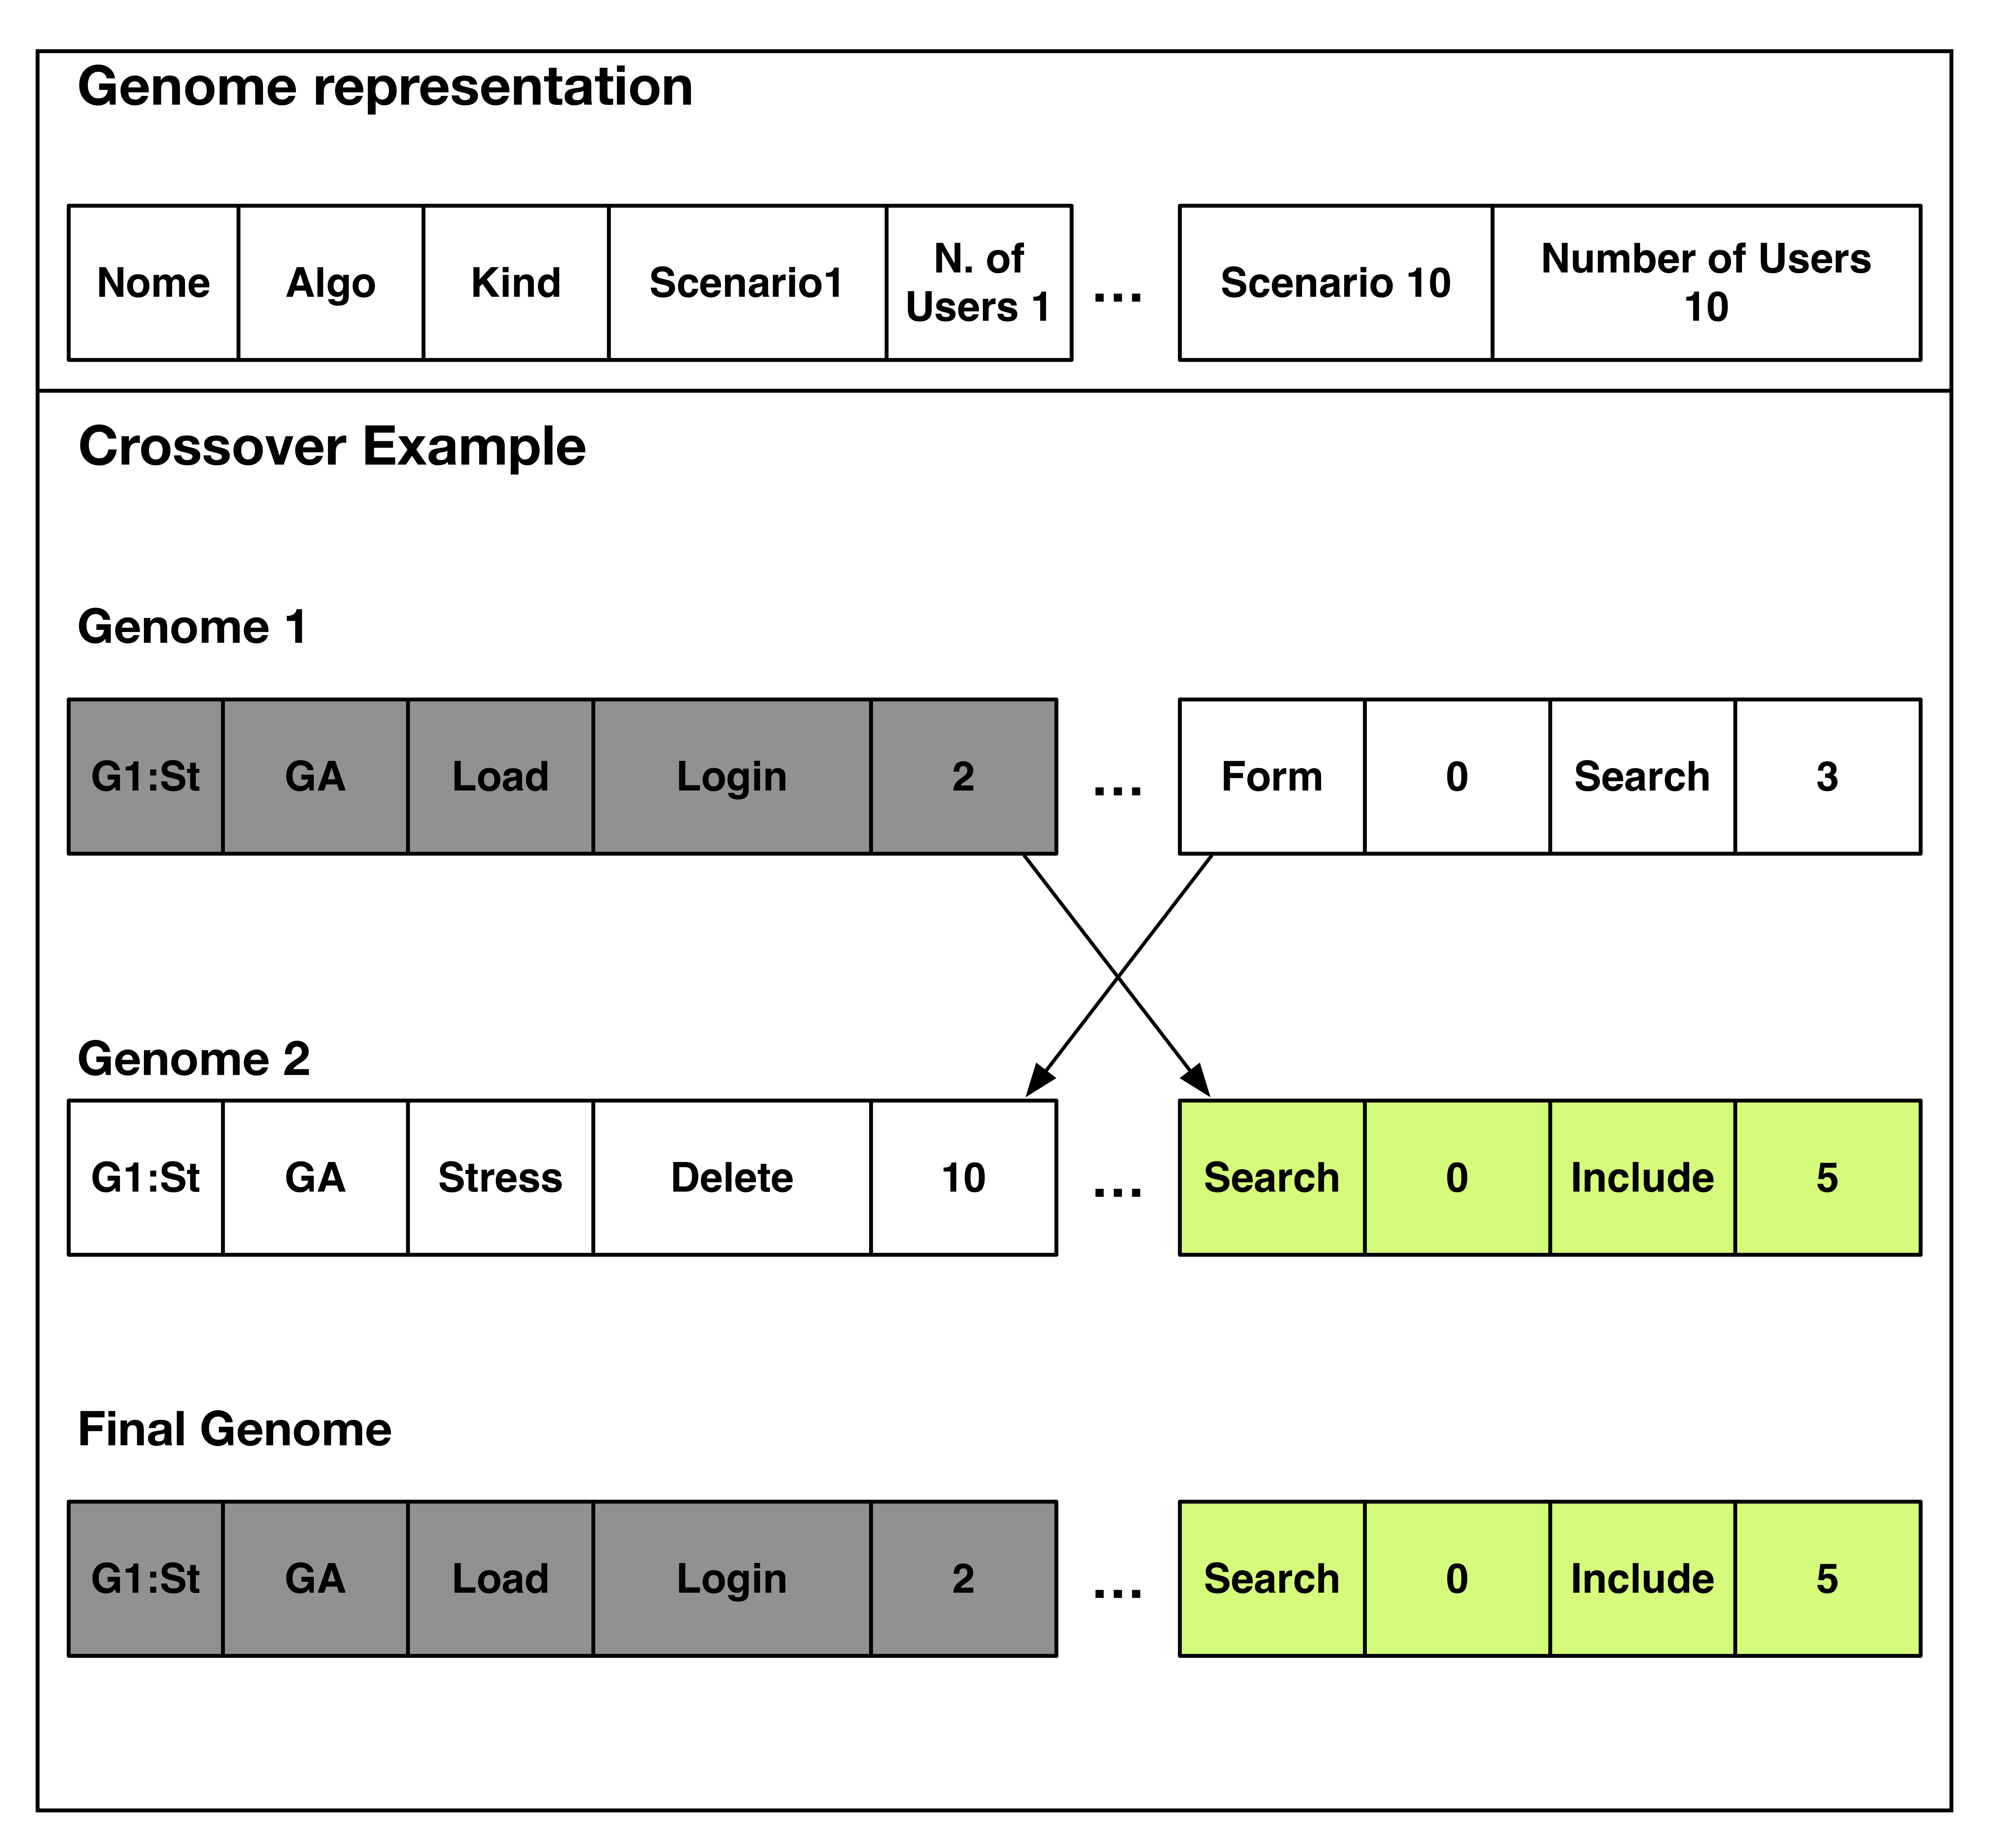
\includegraphics[width=0.5\textwidth]{./images/genomerepresentation.png}
\caption{Genotype representation and crossover example}
\label{fig:genomarepresentation}
\end{figure}

The Fig. \ref{fig:neighbourtaby} shows the strategy used by the IAdapter to obtain the genotype of the neighbours for the Tabu Search and Simulated Annealing algorithms.  The neighbours are obtained by the modification of a single cromossome (scenario or  number of users) in the genotype.

\begin{figure}[h]
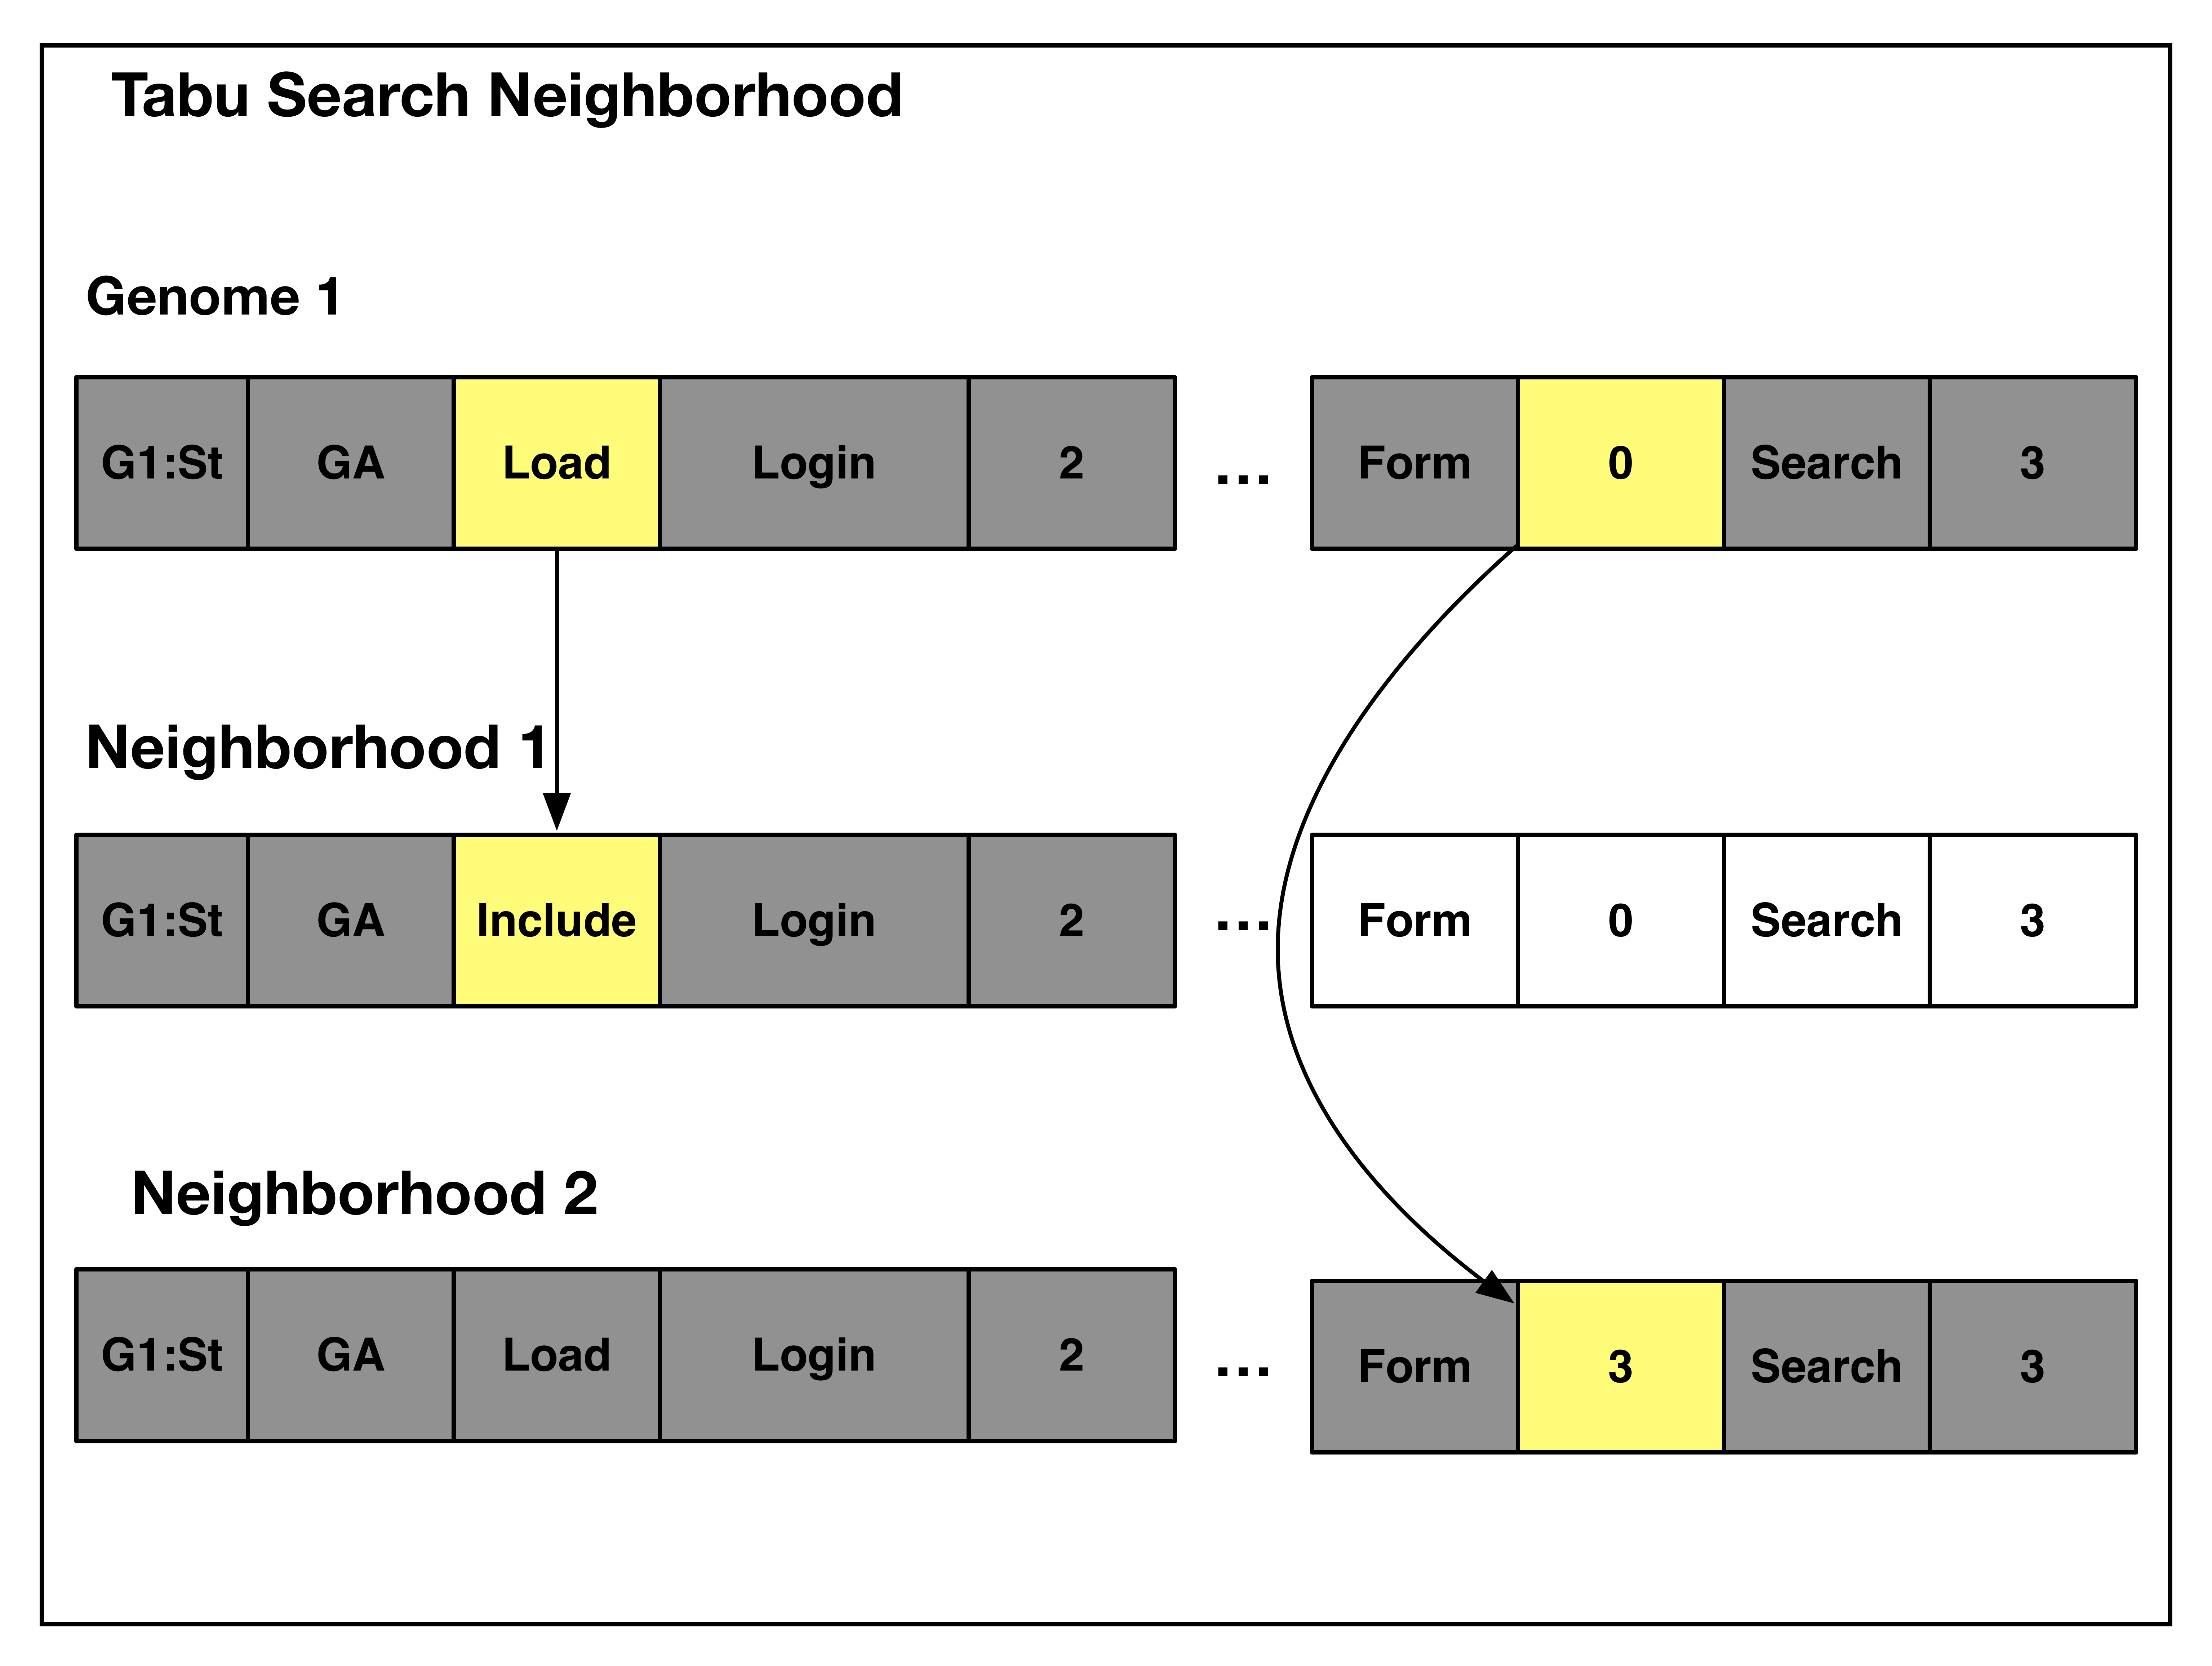
\includegraphics[width=0.5\textwidth]{./images/TabuNE.png}
\caption{Tabu Search and Simulated Annealing neighbour strategy}
\label{fig:neighbourtaby}
\end{figure}


\subsection{Initial population}

The strategy use by the plugin to instantiate the initial population is to generate 50\% of the individuals randomically and 50\% of the initial population are distributed in three  ranges of values:

\begin{itemize}
\item 30\% of the maximum allowed users in the test ;
\item 60\% of the maximum allowed users in the test; and
\item 90\% of the maximum allowed users in the test.
\end{itemize}


\subsection{Objective (Fitnesse) Function}

The proposed solution was designed to be used with the independent testing teams in various situations where the team has no direct access to the environment where the application under test was installed. Therefore,  The IAdapter uses a measurement approach to the definition of the fitnesse function. The fitnesse function applied to IAdapter solution is governed by the following equation:

\begin{equation}
\begin{aligned}
fit=90percentileweigth* 90percentiletime\\
+80percentileweigth*80percentiletime\\+
70percentileweigth*70percentiletime+\\
maxResponseWeigth*maxResponseTime+\\
numberOfUsersWeigth*numberOfUsers-penalty
\end{aligned}
\end{equation}

The proposed solution's fitnesse function uses a series of adaptable user-defined weights ( 90percentileweigth, 80percentileweigth,  70percentileweigth, maxResponseWeigth and numberOfUsersWeigth). These weights make it possible to customize the search plugin functionality. The penalty is applied when a application under test responds in a longer time than the level of service.



